% Generated by Sphinx.
\def\sphinxdocclass{report}
\documentclass[letterpaper,10pt,openany,oneside]{sphinxmanual}
\usepackage[utf8]{inputenc}
\DeclareUnicodeCharacter{00A0}{\nobreakspace}
\usepackage[T1]{fontenc}
\usepackage[english]{babel}
\usepackage{times}
\usepackage[Bjarne]{fncychap}
\usepackage{longtable}
\usepackage{sphinx}
\usepackage{multirow}


\title{Drug Design Exemplar}
\date{March 04, 2014}
\release{}
\author{CSInParallel Project}
\newcommand{\sphinxlogo}{}
\renewcommand{\releasename}{}
\makeindex

\makeatletter
\def\PYG@reset{\let\PYG@it=\relax \let\PYG@bf=\relax%
    \let\PYG@ul=\relax \let\PYG@tc=\relax%
    \let\PYG@bc=\relax \let\PYG@ff=\relax}
\def\PYG@tok#1{\csname PYG@tok@#1\endcsname}
\def\PYG@toks#1+{\ifx\relax#1\empty\else%
    \PYG@tok{#1}\expandafter\PYG@toks\fi}
\def\PYG@do#1{\PYG@bc{\PYG@tc{\PYG@ul{%
    \PYG@it{\PYG@bf{\PYG@ff{#1}}}}}}}
\def\PYG#1#2{\PYG@reset\PYG@toks#1+\relax+\PYG@do{#2}}

\expandafter\def\csname PYG@tok@gd\endcsname{\def\PYG@tc##1{\textcolor[rgb]{0.63,0.00,0.00}{##1}}}
\expandafter\def\csname PYG@tok@gu\endcsname{\let\PYG@bf=\textbf\def\PYG@tc##1{\textcolor[rgb]{0.50,0.00,0.50}{##1}}}
\expandafter\def\csname PYG@tok@gt\endcsname{\def\PYG@tc##1{\textcolor[rgb]{0.00,0.25,0.82}{##1}}}
\expandafter\def\csname PYG@tok@gs\endcsname{\let\PYG@bf=\textbf}
\expandafter\def\csname PYG@tok@gr\endcsname{\def\PYG@tc##1{\textcolor[rgb]{1.00,0.00,0.00}{##1}}}
\expandafter\def\csname PYG@tok@cm\endcsname{\let\PYG@it=\textit\def\PYG@tc##1{\textcolor[rgb]{0.25,0.50,0.56}{##1}}}
\expandafter\def\csname PYG@tok@vg\endcsname{\def\PYG@tc##1{\textcolor[rgb]{0.73,0.38,0.84}{##1}}}
\expandafter\def\csname PYG@tok@m\endcsname{\def\PYG@tc##1{\textcolor[rgb]{0.13,0.50,0.31}{##1}}}
\expandafter\def\csname PYG@tok@mh\endcsname{\def\PYG@tc##1{\textcolor[rgb]{0.13,0.50,0.31}{##1}}}
\expandafter\def\csname PYG@tok@cs\endcsname{\def\PYG@tc##1{\textcolor[rgb]{0.25,0.50,0.56}{##1}}\def\PYG@bc##1{\setlength{\fboxsep}{0pt}\colorbox[rgb]{1.00,0.94,0.94}{\strut ##1}}}
\expandafter\def\csname PYG@tok@ge\endcsname{\let\PYG@it=\textit}
\expandafter\def\csname PYG@tok@vc\endcsname{\def\PYG@tc##1{\textcolor[rgb]{0.73,0.38,0.84}{##1}}}
\expandafter\def\csname PYG@tok@il\endcsname{\def\PYG@tc##1{\textcolor[rgb]{0.13,0.50,0.31}{##1}}}
\expandafter\def\csname PYG@tok@go\endcsname{\def\PYG@tc##1{\textcolor[rgb]{0.19,0.19,0.19}{##1}}}
\expandafter\def\csname PYG@tok@cp\endcsname{\def\PYG@tc##1{\textcolor[rgb]{0.00,0.44,0.13}{##1}}}
\expandafter\def\csname PYG@tok@gi\endcsname{\def\PYG@tc##1{\textcolor[rgb]{0.00,0.63,0.00}{##1}}}
\expandafter\def\csname PYG@tok@gh\endcsname{\let\PYG@bf=\textbf\def\PYG@tc##1{\textcolor[rgb]{0.00,0.00,0.50}{##1}}}
\expandafter\def\csname PYG@tok@ni\endcsname{\let\PYG@bf=\textbf\def\PYG@tc##1{\textcolor[rgb]{0.84,0.33,0.22}{##1}}}
\expandafter\def\csname PYG@tok@nl\endcsname{\let\PYG@bf=\textbf\def\PYG@tc##1{\textcolor[rgb]{0.00,0.13,0.44}{##1}}}
\expandafter\def\csname PYG@tok@nn\endcsname{\let\PYG@bf=\textbf\def\PYG@tc##1{\textcolor[rgb]{0.05,0.52,0.71}{##1}}}
\expandafter\def\csname PYG@tok@no\endcsname{\def\PYG@tc##1{\textcolor[rgb]{0.38,0.68,0.84}{##1}}}
\expandafter\def\csname PYG@tok@na\endcsname{\def\PYG@tc##1{\textcolor[rgb]{0.25,0.44,0.63}{##1}}}
\expandafter\def\csname PYG@tok@nb\endcsname{\def\PYG@tc##1{\textcolor[rgb]{0.00,0.44,0.13}{##1}}}
\expandafter\def\csname PYG@tok@nc\endcsname{\let\PYG@bf=\textbf\def\PYG@tc##1{\textcolor[rgb]{0.05,0.52,0.71}{##1}}}
\expandafter\def\csname PYG@tok@nd\endcsname{\let\PYG@bf=\textbf\def\PYG@tc##1{\textcolor[rgb]{0.33,0.33,0.33}{##1}}}
\expandafter\def\csname PYG@tok@ne\endcsname{\def\PYG@tc##1{\textcolor[rgb]{0.00,0.44,0.13}{##1}}}
\expandafter\def\csname PYG@tok@nf\endcsname{\def\PYG@tc##1{\textcolor[rgb]{0.02,0.16,0.49}{##1}}}
\expandafter\def\csname PYG@tok@si\endcsname{\let\PYG@it=\textit\def\PYG@tc##1{\textcolor[rgb]{0.44,0.63,0.82}{##1}}}
\expandafter\def\csname PYG@tok@s2\endcsname{\def\PYG@tc##1{\textcolor[rgb]{0.25,0.44,0.63}{##1}}}
\expandafter\def\csname PYG@tok@vi\endcsname{\def\PYG@tc##1{\textcolor[rgb]{0.73,0.38,0.84}{##1}}}
\expandafter\def\csname PYG@tok@nt\endcsname{\let\PYG@bf=\textbf\def\PYG@tc##1{\textcolor[rgb]{0.02,0.16,0.45}{##1}}}
\expandafter\def\csname PYG@tok@nv\endcsname{\def\PYG@tc##1{\textcolor[rgb]{0.73,0.38,0.84}{##1}}}
\expandafter\def\csname PYG@tok@s1\endcsname{\def\PYG@tc##1{\textcolor[rgb]{0.25,0.44,0.63}{##1}}}
\expandafter\def\csname PYG@tok@gp\endcsname{\let\PYG@bf=\textbf\def\PYG@tc##1{\textcolor[rgb]{0.78,0.36,0.04}{##1}}}
\expandafter\def\csname PYG@tok@sh\endcsname{\def\PYG@tc##1{\textcolor[rgb]{0.25,0.44,0.63}{##1}}}
\expandafter\def\csname PYG@tok@ow\endcsname{\let\PYG@bf=\textbf\def\PYG@tc##1{\textcolor[rgb]{0.00,0.44,0.13}{##1}}}
\expandafter\def\csname PYG@tok@sx\endcsname{\def\PYG@tc##1{\textcolor[rgb]{0.78,0.36,0.04}{##1}}}
\expandafter\def\csname PYG@tok@bp\endcsname{\def\PYG@tc##1{\textcolor[rgb]{0.00,0.44,0.13}{##1}}}
\expandafter\def\csname PYG@tok@c1\endcsname{\let\PYG@it=\textit\def\PYG@tc##1{\textcolor[rgb]{0.25,0.50,0.56}{##1}}}
\expandafter\def\csname PYG@tok@kc\endcsname{\let\PYG@bf=\textbf\def\PYG@tc##1{\textcolor[rgb]{0.00,0.44,0.13}{##1}}}
\expandafter\def\csname PYG@tok@c\endcsname{\let\PYG@it=\textit\def\PYG@tc##1{\textcolor[rgb]{0.25,0.50,0.56}{##1}}}
\expandafter\def\csname PYG@tok@mf\endcsname{\def\PYG@tc##1{\textcolor[rgb]{0.13,0.50,0.31}{##1}}}
\expandafter\def\csname PYG@tok@err\endcsname{\def\PYG@bc##1{\setlength{\fboxsep}{0pt}\fcolorbox[rgb]{1.00,0.00,0.00}{1,1,1}{\strut ##1}}}
\expandafter\def\csname PYG@tok@kd\endcsname{\let\PYG@bf=\textbf\def\PYG@tc##1{\textcolor[rgb]{0.00,0.44,0.13}{##1}}}
\expandafter\def\csname PYG@tok@ss\endcsname{\def\PYG@tc##1{\textcolor[rgb]{0.32,0.47,0.09}{##1}}}
\expandafter\def\csname PYG@tok@sr\endcsname{\def\PYG@tc##1{\textcolor[rgb]{0.14,0.33,0.53}{##1}}}
\expandafter\def\csname PYG@tok@mo\endcsname{\def\PYG@tc##1{\textcolor[rgb]{0.13,0.50,0.31}{##1}}}
\expandafter\def\csname PYG@tok@mi\endcsname{\def\PYG@tc##1{\textcolor[rgb]{0.13,0.50,0.31}{##1}}}
\expandafter\def\csname PYG@tok@kn\endcsname{\let\PYG@bf=\textbf\def\PYG@tc##1{\textcolor[rgb]{0.00,0.44,0.13}{##1}}}
\expandafter\def\csname PYG@tok@o\endcsname{\def\PYG@tc##1{\textcolor[rgb]{0.40,0.40,0.40}{##1}}}
\expandafter\def\csname PYG@tok@kr\endcsname{\let\PYG@bf=\textbf\def\PYG@tc##1{\textcolor[rgb]{0.00,0.44,0.13}{##1}}}
\expandafter\def\csname PYG@tok@s\endcsname{\def\PYG@tc##1{\textcolor[rgb]{0.25,0.44,0.63}{##1}}}
\expandafter\def\csname PYG@tok@kp\endcsname{\def\PYG@tc##1{\textcolor[rgb]{0.00,0.44,0.13}{##1}}}
\expandafter\def\csname PYG@tok@w\endcsname{\def\PYG@tc##1{\textcolor[rgb]{0.73,0.73,0.73}{##1}}}
\expandafter\def\csname PYG@tok@kt\endcsname{\def\PYG@tc##1{\textcolor[rgb]{0.56,0.13,0.00}{##1}}}
\expandafter\def\csname PYG@tok@sc\endcsname{\def\PYG@tc##1{\textcolor[rgb]{0.25,0.44,0.63}{##1}}}
\expandafter\def\csname PYG@tok@sb\endcsname{\def\PYG@tc##1{\textcolor[rgb]{0.25,0.44,0.63}{##1}}}
\expandafter\def\csname PYG@tok@k\endcsname{\let\PYG@bf=\textbf\def\PYG@tc##1{\textcolor[rgb]{0.00,0.44,0.13}{##1}}}
\expandafter\def\csname PYG@tok@se\endcsname{\let\PYG@bf=\textbf\def\PYG@tc##1{\textcolor[rgb]{0.25,0.44,0.63}{##1}}}
\expandafter\def\csname PYG@tok@sd\endcsname{\let\PYG@it=\textit\def\PYG@tc##1{\textcolor[rgb]{0.25,0.44,0.63}{##1}}}

\def\PYGZbs{\char`\\}
\def\PYGZus{\char`\_}
\def\PYGZob{\char`\{}
\def\PYGZcb{\char`\}}
\def\PYGZca{\char`\^}
\def\PYGZam{\char`\&}
\def\PYGZlt{\char`\<}
\def\PYGZgt{\char`\>}
\def\PYGZsh{\char`\#}
\def\PYGZpc{\char`\%}
\def\PYGZdl{\char`\$}
\def\PYGZti{\char`\~}
% for compatibility with earlier versions
\def\PYGZat{@}
\def\PYGZlb{[}
\def\PYGZrb{]}
\makeatother

\begin{document}

\maketitle
\tableofcontents
\phantomsection\label{index::doc}


In this document we present a problem from molecular biology and chemistry that requires computation to solve.  The real-world problem is fairly complex.  Here we simplify it to present the essence of the problem being solved.  We call this problem description and it solutions an \emph{exemplar} of the original real-world computation.  In this document we introduce the problem and provide one form of sequential programmed solution.  In a follow-up document there are parallel programming solutions using different languages and computing hardware and software.


\chapter{Introduction}
\label{intro/intro:introduction}\label{intro/intro:drug-design-exemplar}\label{intro/intro::doc}

\section{Background: Drug Design}
\label{intro/intro:background-drug-design}
An important problem in the biological sciences is that of drug design. The goal is to find small molecules, called \emph{ligands}, that are good candidates for use as drugs.
\begin{quote}
\begin{figure}[htbp]
\centering

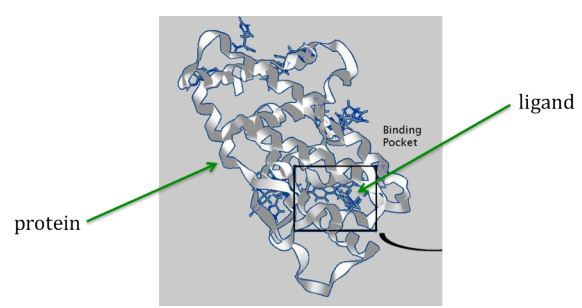
\includegraphics{proteinligand.jpg}
\end{figure}
\begin{quote}\begin{description}
\item[{width}] \leavevmode
582px

\item[{align}] \leavevmode
center

\item[{height}] \leavevmode
308px

\item[{alt}] \leavevmode
Diagram of a ligand binding to a protein.

\item[{figclass}] \leavevmode
align-center

\end{description}\end{quote}
\end{quote}

At a high level, the problem is simple to state: a protein associated with the disease of interest is identified, and its three-dimensional structure is found either experimentally or through a molecular modeling computation. A collection of ligands is tested against the protein: for example, for every orientation of the ligand relative to the protein, computation is done to test whether the ligand binds with the protein in useful ways (such as tying up a biologically active region on the protein). A score is set based on these binding properties, and the best scores are flagged, identifying ligands that would make good drug candidates.


\section{Algorithmic Strategy}
\label{intro/intro:algorithmic-strategy}
We will apply a \emph{map-reduce} strategy to this problem, which can be implemented using a \emph{master-worker} design pattern.

Our map-reduce strategy uses three stages of processing.
\begin{enumerate}
\item {} 
First, we will generate many ligands to be tested agains a given protein, using a function \code{Generate\_tasks().} This function produces many \code{{[}ligand, protein{]}} pairs (in this case, all with the same protein) for the next stage.

\item {} 
Next, we will apply a \code{Map()} function to each ligand and the given protein,       which will compute the binding score for that \code{{[}ligand, protein{]}} pair. This \code{Map()} function will produce a pair \code{{[}score, ligand{]}} since we want to know the highest-scoring ligands.

\item {} 
Finally, we identify the ligands with the highest scores, using a function \code{Reduce()} applied to the \code{{[}score, ligand{]}} pairs.

\end{enumerate}

These functions could be implemented sequentially, or they can be called by multiple processes or threads to perform the drug-design computation in parallel: one process, called the \emph{master}, can fill a task queue with pairs obtained from \code{Generate\_tasks().}
Many \emph{worker} processes can pull tasks off the task queue and apply the function \code{Map()} to them. The master can then collect results from the workers and apply \code{Reduce()} to determine the highest-scoring ligand(s).

Note that if the \code{Reduce()} function is expensive to apply, or if the stream of \code{{[}score, ligand{]}} pairs produced by calls to \code{Map()} becomes too large, the \code{Reduce()} stage may be parallelized as well.

This map-reduce approach has been used on clusters and large \href{http://en.wikipedia.org/wiki/Non-Uniform\_Memory\_Access}{NUMA} machines. Stanford University's \href{http://folding.stanford.edu/}{Folding@home} project also involves using idle processing resources from thousands of volunteers' personal computers to run computations on protein folding and related diseases.


\chapter{A Sequential Solution}
\label{sequentialimplementation/sequentialimplementation:a-sequential-solution}\label{sequentialimplementation/sequentialimplementation::doc}\label{sequentialimplementation/sequentialimplementation:folding-home}

\section{Problem Definition}
\label{sequentialimplementation/sequentialimplementation:problem-definition}
Working with actual ligand and protein data is beyond the scope of this example, so we will represent the computation by a simpler string-based comparison.

Specifically, we simplify the computation as follows:
\begin{quote}
\begin{itemize}
\item {} 
Proteins and ligands will be represented as (randomly-generated) character strings.

\item {} 
The docking-problem computation will be represented by comparing a ligand string \code{L} to a protein string \code{P}.  The score for a pair \code{{[}L, P{]}} will be the maximum number of matching characters among all possibilities when \code{L} is compared to \code{P}, moving from left to right, allowing possible insertions and deletions.  For example, if \code{L} is the string “cxtbcrv” and \code{P} is the string “lcacxtqvivg,” then the score is 4, arising from this comparison of \code{L} to a segment of \code{P}:

\end{itemize}
\begin{figure}[htbp]
\centering

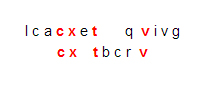
\includegraphics{seq1.jpg}
\end{figure}
\end{quote}

This is not the only comparison of that ligand to that protein that yields four matching characters. Another one is
\begin{quote}
\begin{figure}[htbp]
\centering

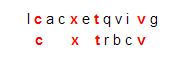
\includegraphics{seq2.jpg}
\end{figure}
\end{quote}

However, there is no comparison that matches five characters while moving from left to right, so the score is 4.


\section{Implementation}
\label{sequentialimplementation/sequentialimplementation:implementation}
The example program \code{dd\_serial.cpp} provides a sequential C++ implementation of our simplified drug design problem.
\begin{quote}

\begin{notice}{note}{Note:}
The program optionally accepts up to three command-line arguments:
\begin{enumerate}
\item {} 
maximum length of the (randomly generated) ligand strings

\item {} 
number of ligands generated

\item {} 
protein string to which ligands will be compared

\end{enumerate}
\end{notice}
\end{quote}


\subsection{The Code}
\label{sequentialimplementation/sequentialimplementation:the-code}
In this implementation, the class \code{MR} encapsulates the map-reduce steps \code{Generate\_tasks()}, \code{Map()}, and \code{Reduce()} as private methods (member functions of the class), and a public method \code{run()} invokes those steps according to a map-reduce algorithmic strategy (see above for detailed explanation). We have highlighted calls to the methods representing map-reduce steps in the following code segment from \code{MR::run()}.
\begin{quote}

\begin{Verbatim}[commandchars=\\\{\},numbers=left,firstnumber=1,stepnumber=1]
\PYG{n}{Generate\PYGZus{}tasks}\PYG{p}{(}\PYG{n}{tasks}\PYG{p}{)}\PYG{p}{;}
\PYG{c+c1}{// assert -- tasks is non-empty}

\PYG{k}{while} \PYG{p}{(}\PYG{o}{!}\PYG{n}{tasks}\PYG{p}{.}\PYG{n}{empty}\PYG{p}{(}\PYG{p}{)}\PYG{p}{)} \PYG{p}{\PYGZob{}}
  \PYG{n}{Map}\PYG{p}{(}\PYG{n}{tasks}\PYG{p}{.}\PYG{n}{front}\PYG{p}{(}\PYG{p}{)}\PYG{p}{,} \PYG{n}{pairs}\PYG{p}{)}\PYG{p}{;}
  \PYG{n}{tasks}\PYG{p}{.}\PYG{n}{pop}\PYG{p}{(}\PYG{p}{)}\PYG{p}{;}
\PYG{p}{\PYGZcb{}}

\PYG{n}{do\PYGZus{}sort}\PYG{p}{(}\PYG{n}{pairs}\PYG{p}{)}\PYG{p}{;}

\PYG{k+kt}{int} \PYG{n}{next} \PYG{o}{=} \PYG{l+m+mi}{0}\PYG{p}{;}  \PYG{c+c1}{// index of first unprocessed pair in pairs[]}
\PYG{k}{while} \PYG{p}{(}\PYG{n}{next} \PYG{o}{\PYGZlt{}} \PYG{n}{pairs}\PYG{p}{.}\PYG{n}{size}\PYG{p}{(}\PYG{p}{)}\PYG{p}{)} \PYG{p}{\PYGZob{}}
  \PYG{n}{string} \PYG{n}{values}\PYG{p}{;}
  \PYG{n}{values} \PYG{o}{=} \PYG{l+s}{"}\PYG{l+s}{"}\PYG{p}{;}
  \PYG{k+kt}{int} \PYG{n}{key} \PYG{o}{=} \PYG{n}{pairs}\PYG{p}{[}\PYG{n}{next}\PYG{p}{]}\PYG{p}{.}\PYG{n}{key}\PYG{p}{;}
  \PYG{n}{next} \PYG{o}{=} \PYG{n}{Reduce}\PYG{p}{(}\PYG{n}{key}\PYG{p}{,} \PYG{n}{pairs}\PYG{p}{,} \PYG{n}{next}\PYG{p}{,} \PYG{n}{values}\PYG{p}{)}\PYG{p}{;}
  \PYG{n}{Pair} \PYG{n}{p}\PYG{p}{(}\PYG{n}{key}\PYG{p}{,} \PYG{n}{values}\PYG{p}{)}\PYG{p}{;}
  \PYG{n}{results}\PYG{p}{.}\PYG{n}{push\PYGZus{}back}\PYG{p}{(}\PYG{n}{p}\PYG{p}{)}\PYG{p}{;}
\PYG{p}{\PYGZcb{}}
\end{Verbatim}
\end{quote}


\subsection{Comments}
\label{sequentialimplementation/sequentialimplementation:comments}\begin{itemize}
\item {} 
We use the \href{http://www.cplusplus.com/reference/stl/}{STL containers}  \code{queue\textless{}\textgreater{}}  and  \code{vector\textless{}\textgreater{}}  to hold the results from each of the map-reduce steps: namely, the task queue of ligands to process, the list key-value pairs produced by the \code{Map()} phase, and the list of resulting key-value pairs produced by calls to \code{Reduce()}. We define those container variables as data members in the class \code{MR}:
\begin{quote}

\code{queue\textless{}string\textgreater{} tasks;}

\code{vector\textless{}Pair\textgreater{} pairs, results;}
\end{quote}

\item {} 
Here, \code{Pair} is a struct representing key-value pairs with the desired types:

\begin{Verbatim}[commandchars=\\\{\},numbers=left,firstnumber=1,stepnumber=1]
\PYG{k}{struct} \PYG{n}{Pair} \PYG{p}{\PYGZob{}}
  \PYG{k+kt}{int} \PYG{n}{key}\PYG{p}{;}
  \PYG{n}{string} \PYG{n}{val}\PYG{p}{;}
  \PYG{n}{Pair}\PYG{p}{(}\PYG{k+kt}{int} \PYG{n}{k}\PYG{p}{,} \PYG{k}{const} \PYG{n}{string} \PYG{o}{\PYGZam{}}\PYG{n}{v}\PYG{p}{)} \PYG{p}{\PYGZob{}}\PYG{n}{key}\PYG{o}{=}\PYG{n}{k}\PYG{p}{;} \PYG{n}{val}\PYG{o}{=}\PYG{n}{v}\PYG{p}{;}\PYG{p}{\PYGZcb{}}
\PYG{p}{\PYGZcb{}}\PYG{p}{;}
\end{Verbatim}

\item {} 
In the example code, \code{Generate\_tasks()} merely produces \emph{nligands} strings of random lower-case letters, each having a random length between 0 and \emph{max\_ligand}. The program stores those strings in a task queue named \code{tasks}.

\item {} 
For each ligand in the task queue, the \code{Map()} function computes the match score from comparing a string representing that ligand to a global string representing a target protein, using the simplified match-scoring algorithm described above. \code{Map()} then yields a key-value pair consisting of that score and that ligand, respectively.

\item {} 
The key-value pairs produced by all calls to \code{Map()} are sorted by key in order to group pairs with the same score. Then \code{Reduce()} is called once for each of those groups in order to yield a vector of \code{Pairs} consisting of a score \emph{s} together with a list of all ligands whose best score was \emph{s}.

\begin{notice}{note}{Note:}
Map-reduce frameworks such as the open-source Hadoop commonly use sorting to group values for a given key, as does our program. This has the additional benefit of producing sorted results from the reduce stage. Also, the staged processes of performing all \code{Map()} calls before sorting and of performing all \code{Reduce()} calls after the completion of sorting are also common among map-reduce frameworks.
\end{notice}

\item {} 
The methods \code{Generate\_tasks()}, \code{Map()}, and \code{Reduce()} may seem like unnecessary complication for this problem since they abstract so little code. Indeed, we could certainly rewrite the program more simply and briefly without them. We chose this expression for several reasons:
\begin{itemize}
\item {} 
We can compare code segments from \code{MR::run()} directly with corresponding segments in upcoming parallel implementations to focus on the parallelization changes and hide the common code in method calls.

\item {} 
The methods \code{Generate\_tasks()}, \code{Map()}, and \code{Reduce()} make it obvious where to insert more realistic task generation, docking algorithm, etc., and where to change our map-reduce code examples for problems other than drug design.

\item {} 
We use these three method names in descriptions of the map-reduce pattern elsewhere.

\end{itemize}

\item {} 
We have not attempted to implement the fault tolerance and scalability features of a production map-reduce framework such as Hadoop.

\end{itemize}


\subsection{Questions for Exploration}
\label{sequentialimplementation/sequentialimplementation:questions-for-exploration}\label{sequentialimplementation/sequentialimplementation:stl-containers}\begin{itemize}
\item {} 
Compile and test run the sequential program. Determine values for the command-line arguments \code{max\_ligand{}`{}`(maximum length of a ligand string) and {}`{}`nligands} (total number of ligands to process) that lead to a tolerably long computation for experimenting (e.g., perhaps 15 seconds to a minute of computation). Note the following about our simplified computational problem:
\begin{itemize}
\item {} 
Our stand-in scoring algorithm is exponential in the lengths of the ligand and protein strings. Thus, a large value of \code{max\_ligand} may cause an extremely lengthy computation. Altering \code{max\_ligand} can help in finding a test computation of a desired order of magnitude.

\item {} 
We expect the computation time to increase approximately linearly with the number of ligands \code{nligands}. However, if \code{nligands} is relatively small, you may notice irregular jumps to long computation times when increasing \code{nligands}. This is because our simple random algorithm for generating ligands produces ligand strings using \code{random()}, as well as ligands with random lengths as well as random content.  Because of the order-of-magnitude effect of ligand length, a sudden long ligand (meaning more characters than those before) may greatly increase the computation time.

\end{itemize}

\item {} 
If you have \emph{more realistic algorithms for docking and/or more realistic data for ligands and proteins}, modify the program to incorporate those elements, and compare the results from your modified program to results obtained by other means (other software, wet-lab results, etc.).

\end{itemize}



\renewcommand{\indexname}{Index}
\printindex
\end{document}
